\documentclass[]{article}
\usepackage[margin=1in]{geometry}
\usepackage{amsmath}
\usepackage{cite}
\usepackage{refstyle}
\usepackage{caption}
\usepackage{float}
\usepackage{graphicx}
%opening
\title{\vspace{-25mm} Edge Detection using Adaptive Mean Filtering}
\date{}
\author{
	Tanmay Gulati\\
	\texttt{160905320}\\
	\texttt{VI - C : 48}\\
	\and
	Shiven Sharma\\
	\texttt{160905386}\\
	\texttt{VI - C : 60}\\
	\and
	Yash Raj Sarrof\\
	\texttt{160905390}\\
	\texttt{VI - C : 61}
}
\begin{document}
\pagestyle{empty}
\maketitle
\section*{Abstract} 
\hspace{6mm} In simple thresholding, the threshold value is global, i.e., it is same for all the pixels in the image.
Adaptive thresholding is the method where the threshold value is calculated for smaller regions and
therefore, there will be different threshold values for different regions. The Wiener filtering executes an
optimal tradeoff between inverse filtering and noise smoothing. It removes the additive noise and inverts
the blurring simultaneously

\section*{Objective} 
\hspace{6mm} Parallelize the Adaptive edge detection process done using Weiner filter, demonstrate in both CUDA and MPI. The main motivation is to remove noise from the image, then apply any of the commonly known filters to detect images. We apply sobel filter to find horizontal edges. Although the only difference to the algorithm to find vertical edges, would be to take the transpose of the filter and use that as the base filter instead. 

\section*{Introduction}
\hspace{6mm} Edge detection refers to the process of identifying and locating sharp discontinuities in an image. The discontinuities are abrupt changes in pixel intensity which characterize boundaries of objects in a scene. Classical
methods of edge detection involve convolving the image with an operator (a 2-D filter), which is constructed
to be sensitive to large gradients in the image while returning values of zero in uniform regions.
Variables involved in the selection of an edge detection operator includes : \\
\textbullet \hspace{4mm} Edge orientation (horizontal/vertical) \\
\textbullet  \hspace{4mm} Amount of Noise in environment\\
\textbullet \hspace{4mm}  Edge Structure (steep change in intensity at edge/gradual change in intensity)\\

\hspace{4mm}Gradient-based algorithms such as the Prewitt filter have a major drawback of being very sensitive to
noise. The size of the kernel filter and coefficients are fixed and cannot be adapted to a given image. An
adaptive edge-detection algorithm is necessary to provide a robust solution that is adaptable to the varying
noise levels and Weiner Filter provides for one such solution.
\section*{Literature Review}
The base paper for this project \cite{woodhall1997new} takes a concept of signal processing i.e. adaptive mean filtering and applies that to a common application in image processing, which is edge detection. Adaptive mean filtering is standard technique of reducing noise in signal processing. In \cite{weib1998adaptive}, various variations of mean filtering can be found, and thus different variations to this filtering method can be applied for this application as well. A performance analysis of such varied methods has been done comprehensively in \cite{bitmead1980performance}. This algorithm was one of the earliest developments in image processing, and more recent versions of Weiner filter can be found as well as in \cite{chen2006new}. Also, parallel implementations of this algorithm have been done as well, like in \cite{allred2003implementation}, where LMS filter is used on some superscalar architecture.
\section*{Methodology}
The following steps need to be followed to implement the algorithm. Parallelizing in CUDA is done at pixel level, however with MPI it is done at the row level, where each row concurrently gets executed. Since the number of threads required for a pixel level computation is not supported by MPI. Unless specified, all the steps are parallelized in the same manner as stated above.\\

\textbullet \hspace{4mm} The image needs to be read into our programs for both CUDA and MPI, since we are using C as our base language, this is done through a publicly available library named \textbf{stb\_image.h}. The library function returns the image in a 1D character array. We do all the necessary declarations here itself. It should be noted that this part of the algorithm cannot be parallelized in any way whatsover. \\

\textbullet \hspace{4mm} Since the image is in character array, we need to cast all the elements to an integer, so that arithmetic operations can be performed on the images. The final 1D integer array is stored as \textbf{image}. \\

\textbullet \hspace{4mm} The input image is padded with 1 layer of 0 intensity pixels. The same is done by having the whole image copied into a new 1-D array of length \textbf{(row+1)*(col+1)}, with the first, last column and row
made as 0, others having intensity values of the original image with the mapping \textbf{ image\_pad[(i)*(cols+1) + j] = image[(i-1)*cols + (j-1)] } \\

\textbullet \hspace{4mm} Compute the local means and local variances of the pixels of the input image, by considering a neighbourhood of 3*3, and store it in the 1D arrays of \textbf{localmean} and \textbf{localvariance}. \\

\textbullet \hspace{4mm} Find the global variance of the image as a whole and store it in the variable \textbf{variance} Using which \textbf{localvariance} array is modified to be greater than at least the global variance, i.e. \textbf{variance}. \\

\textbullet \hspace{4mm} Inverse adaptive mean filtering is applied to the image, with the following equation being applied to each and every pixel in the image, and output is stored in \textbf{filtered}. 

\begin{equation}
filtered[i*cols + j] = image[i*cols+j] - \frac{variance}{localvariance[i*cols+j]}*( image[i*cols+j] - localmean[i*cols+j]) 
\end{equation} \\

\textbullet \hspace{4mm} Convolve any filter meant to be used for edge detection to the padded version of the filtered image. For demonstration, we have used a horizontal sobel filter.  \\

\textbullet \hspace{4mm} Finally, again since we are using C, we need to save the image with the detected images. The same is done through a publicly licensed library \textbf{stb\_image\_write.h}. Again this can only save character arrays, thus the image is casted to a char, and the final image is saved as \textbf{final\_image.h}.


\section*{Results} 
\hspace{4mm} On an average the runtime of the overall algorithm is reduced by about 60-70\% , while using CUDA, and about 
25 - 30 \% while using MPI. The difference is a result of the fact that we are not able to make as many threads in
MPI as in CUDA. Thus whereas we make all the pixels of the image directly compute steps on it's own in CUDA. In MPI only 
the rows or the columns of the image can be parallelized.\\
A sample input in \figref{input} and corresponding output in \figref{output} is shown here. Thus the algorithm definitely works well for images with no noise. \\ \\ \\
\begin{figure}[H]
	
\includegraphics[scale=0.25]{logo.png}
	\centering
	\caption{Clean Input Image} 
	\label{fig:input}
\end{figure}
\begin{figure}[H]
	\centering
	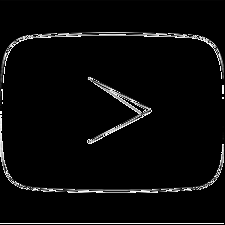
\includegraphics[scale=0.25]{image.png}
	\caption{Output Image with horizontal edges}
	\label{fig:output}
\end{figure}

\vspace{5mm} However looking at \figref{inputnoise} , the algorithm manages to detect edges and higlights even in highly noisy images as can be seen in \figref{outputnoise}.  Thus if edge detection is part of a preprocessing step, it would help a lot of applications, in the sense that the immense processing power of a GPU could be used for more advanced applications.\\ \\ \\ 
\begin{figure}[H]
	\includegraphics[scale=0.25]{sp_noise.png}
	\centering
	\caption{Input Image with noise} 
	\label{fig:inputnoise}
\end{figure}
\begin{figure}[H]
	\centering
	\includegraphics[scale=0.25]{detect.png}
	\caption{Output Image}
	\label{fig:outputnoise}
\end{figure}

\vspace{5mm}
\section*{Limitations and Possible Improvements}
\hspace{4mm} For the purposes of this project the filter size has not been tampererd, varying filter sizes could provide
for better results. Also, the accuracy of the algorithm severely depends on the function taken for making
the image more immune to the noise and is now, probably too outdated to be used in mainstream applications. 
Especially with the boom of deep learning and the excellent results achieved with convolution neural
networks, it would make better sense to use that for any image processing applications with GPU and fast
processing available at hand, since the potential trade off achieved in favour of time, does not justify using
this algorithm anymore. Another area of improvement could come up in adding more feature engineering,
and improving the algorithm to parallelize further.
\section*{Conclusion}
\hspace{4mm} Adaptive Mean filtering, and using that to negate the effect of noise although works well, but with other
alternatives opening up to negate noise, it has almost lost relevance, and in case the noise is not all that
much, then using a fixed filter makes much more sense, since the computations are far lesser. However, it
can still be used as part of preprocessing.

\bibliography{refer} 
\bibliographystyle{ieeetr}


\end{document}
